\begin{titlepage}
    \centering
    %\vspace*{0.5 cm}
    
\includegraphics[scale = 0.4]{Config/uon.png}\\[1.0 cm]	% University Logo

    
    \textsc{\Large Department of Electrical and Electronic Engineering
    Faculty of Engineering}\\[0.5 cm]	% University Name
    \textsc{\large EEE Final Year Individual Project}\\[0.5 cm]				% Course Code
    \textsc{\large (EEEE4008 UNUK FYR) (24-25)}\\[0.5 cm]				% Course Name

    \rule{\linewidth}{0.2 mm} \\[0.4 cm]
    { \huge \bfseries \thetitle}\\
    \rule{\linewidth}{0.2 mm} \\[0.5 cm]

    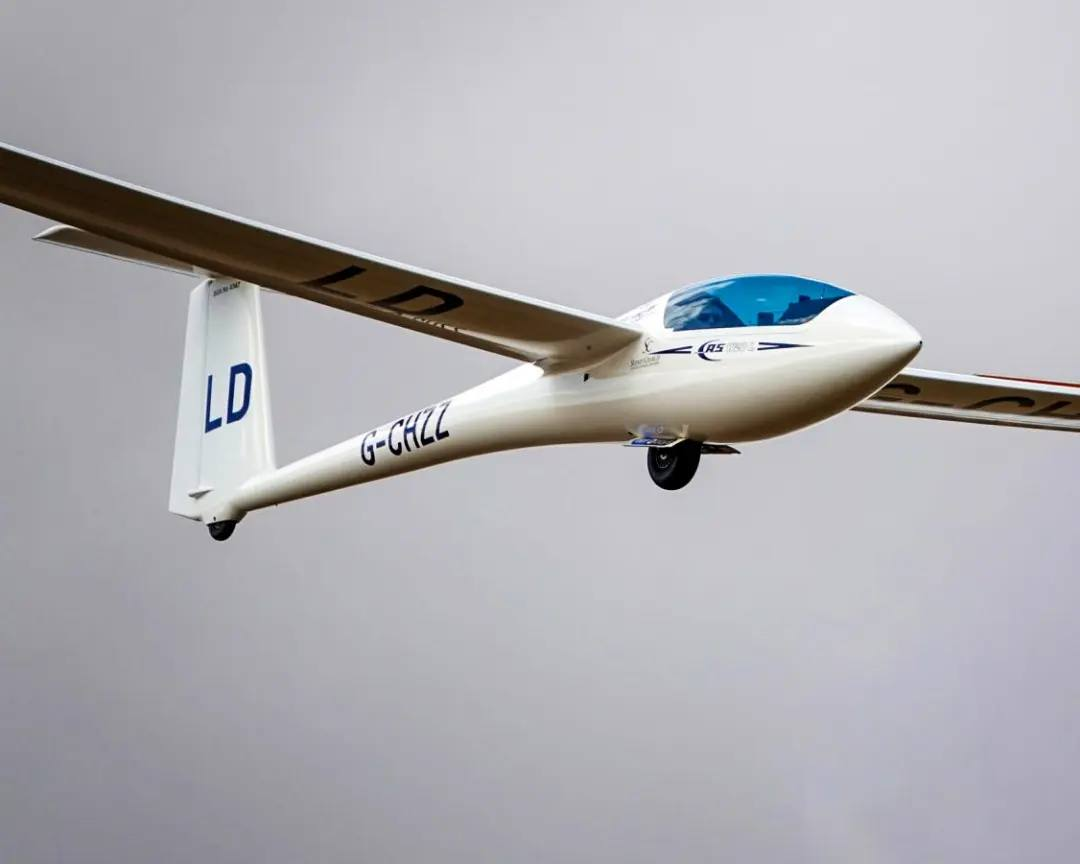
\includegraphics[scale = 0.3]{Config/a.jpg}\\[1.0 cm]

    \large \emph{Author:} \theauthor \\[0.5 cm]


    {\large \thedate}\\[0 cm]

    \vfill

\end{titlepage}

% \section{Overleaf Hints (to be deleted later)}

% \subsection{jumping between doc and latex}
% use ctr+click to jump in pages. \\

% use ctr+S to compile document.


% \subsection{Drawings}
% make drawings with: https://www.mathcha.io/editor/ \\


% \subsection{Graphs}
% all graphs should be done in matlab. Use matlab2tikz to create a latex file:

% https://uk.mathworks.com/matlabcentral/fileexchange/22022-matlab2tikz-matlab2tikz

% use the command to add your graph: 
% \begin{verbatim}
%         \input{path/to/your/file.tex}
% \end{verbatim}  

% This should be wrapped in a figure see \cref{sub:figures}

% \subsection{Tables}
% to make tables use: 
% https://www.tablesgenerator.com/

% use the [ht!] flag to specify table position.\\

% use following to ensure it stays in bounds
% \begin{verbatim}
%     \centering
%     \resizebox{\columnwidth}{!}
% \end{verbatim}

% if wraparound boxes are needed use:
% \begin{verbatim}
%     \tabular{p{100}} where p 100 is in pt.
% \end{verbatim}\\

% see \cref{tab:inital_spec_vs_Considerations} for example\\

% \subsection{Peer Review process}
% leave in green, for someone else to read. don't click accept on your own work \\

% if you see green that is not your own work. review it, then accept it. make sure to use a spell checker (you can get Grammarly for overleaf)\\

% \subsection{figures} \label{sub:figures}
% please use the following template for figures:

% \begin{figure}[ht!]
%     \centering
%     % \includegraphics{}
%     \caption{Caption}
%     \label{fig:enter-label}
% \end{figure}


% \subsection{referencing}
% \subsubsection{Cross referencing}

% use \verb|\Cref and \cref| ... eg \Cref{tab:inital_spec_vs_Considerations} and \cref{tab:inital_spec_vs_Considerations}

% label where appropriate:

% eg: \verb|\label{fig:figure_descritpion}| or \verb|\label{tab:table_description}| or \verb|\label{sec:section_name}|

% \subsubsection{citations}

% get extension BibItNow:

% https://addons.mozilla.org/en-US/firefox/addon/bibitnow/

% copy reference in bibtex format.

% paste in file biblist.bib found in the main file tree near bottom.

% eg:

% \begin{verbatim}
%     @misc{CanoeSlalom,
% 	title = {{Canoe Slalom}},
% 	journal = {ICF - Planet Canoe},
% 	year = {2023},
% 	month = oct,
% 	note = {[Online; accessed 31. Oct. 2023]},
% 	url = {https://www.canoeicf.com/disciplines/canoe-slalom}
% }
% \end{verbatim}


% Then use \verb|\cite{CanoeSlalom}| to reference: \cite{CanoeSlalom}

% if done correctly it should automatically appear hyper linked to the bottom of the document.



% \pagebreak
% \vspace*{\fill}
% \begin{abstract}
%    This report will discuss the feasibility of creating a full slalom canoe and kayak timing and scoring systems to automate the adjudication of the water sport. The report investigates the background and context behind the sport, including looking at existing solutions and analysing where similar automation has been achieved in other sporting disciplines. The stakeholder's requirements have been analysed qualitatively and quantitatively to generate a set of specifications for initial idea generation. An IoT radio localisation system has been conceptualised to map, track and report the athlete's position in time and space. Satellite nodes on each pole contain sensors to detect hits and act as radio beacons for localisation and data communication. An offline computer processes this data to generate scoring and timing data, displayed in real-time to a spectator through an app. Subsystems for rover and satellite prototypes, as well as a prototype scoring system and application, were implemented and tested. The prototypes were analysed against the specifications and original stakeholder requirements. Reflections were made on all aspects of the project and the project as a whole, including project management. Areas for future work and further development proposed. Broader context and commercialisation strategies were discussed to extrapolate the work's long-term implications. 
% \end{abstract}
% \vspace*{\fill}
% \pagebreak